\documentclass[a4paper, 12pt]{article}
\usepackage{cmap}
\usepackage[utf8]{inputenc}
\usepackage[english, russian]{babel}
\usepackage[left=2cm, right=2cm, top=2cm, bottom=2cm]{geometry}
\usepackage{amsfonts,amssymb}
\usepackage{amsmath}
\usepackage{amsthm}
\usepackage{titlesec}
\usepackage{graphicx}
\usepackage{mathtools}

 \newcommand{\tit}[1]{\begin{center}{\bf{\Large #1}}\end{center}}
 \newcommand{\aut}[1]{\centerline{{\bf #1}}}
 \newcommand{\cityorg}[1]{\centerline{\it #1}}
 \newcommand{\email}[1]{\centerline{{\small e-mail: #1}}\vspace{\baselineskip}}
\providecommand{\keywords}[1]{\textbf{\textit{Ключевые слова:}} #1}
\newcommand{\norm}[1]{\left\lVert#1\right\rVert}
\newcommand{\normb}[1]{\left\lVert\textbf{#1}\right\rVert}
\newtheorem{lemma}{Лемма}
\begin{document}

\sloppy

 \tit{Идеальная цилиндрическая оболочка: совершенная, но чувствительная к малым возмущениям}
 \tit{Ideal Cylindrical Cloak: Perfect but Sensitive to Tiny Perturbations}
 \aut{Zhichao Ruan, Min Yan, Curtis W. Neff, and Min Qiu}
 \cityorg{Laboratory of Optics, Photonics and Quantum Electronics,} 
 \cityorg{Department of Microelectronics and Applied Physics,} 
 \cityorg{Royal Institute of Technology (KTH), Electrum 229, 16440 Kista, Sweden}
 \cityorg{Joint Research Center of Photonics of the}
 \cityorg{Royal Institute of Technology (Sweden) and Zhejiang University,}
 \cityorg{Zhejiang University, Yu-Quan, 310027 Hangzhou, People’s Republic of China}
 \email{min@kth.se}

\begin{abstract}
\end{abstract}

В последних работах обсуждался захватывающий вопрос экзотичесих материалов, невидимых для электромагнитных волн
(EM) \cite{1}-\cite{11}. Основываясь на преобразовании координат в уравнениях Максвелла Пендри и другие впервые
предложили мантию невидивку, которая может защищать объект внутри нее от обнаружения \cite{1}: когда 
электромагнитные волны проходят сквозь мантию невидимку, она отражает их, направляя вокруг объекта, затем
возвращает в первоначальное направление, не возмущая внешнее поле. Также недавно сообщалось о численных методах,
примененных для решения задачи EM, включающаю плащ невидимку \cite{6,9}, и экспериментальных результатов 
маскировки с использованием метаматериалов с упрощенными параметрами \cite{7}. Тем не менее, идеальный плащ-
невидимка не была подтверждена как совершенная оболочка, в связи с экстримальными физическими параметрами (ноль 
или бесконечность) в идеальной оболочке при приближении к внутренней границе.

В этой работе мы рассмотрим рассеяние идеального плаща-невидимки. Мы сфокусируем наш анализ на двумерной циллиндрической
оболочке, поскольку волновое уравнение, по сравнению с трехмерным случаем может быть упрощено, так же двумерную оболочку
более проще изготовить \cite{7}. Мы воспользуемся приемуществом цилиндрической геометрии структуры и используем
метод расширения цилиндрической волны для изучения устройства полуаналитически. Чтобы избежать экстремальных значений
(нуля или бесконечности), мы введем небольшое возмущение в идеальную оболочку и позволим ему достигнуть нуля, чтобы
изучить задачу рассеяния для идеальной оболочки. Такой асимптотический анализ может показать не только, является ли
идеально невидимой или нет, но и предоставляет подсказки, насколько чувствительно такое устройство к конечным 
возмущениям. Анализ чувствительности плаща-невидимки прямо определяет возможно его применения. Наши исследования 
показывают, что цилиндическая оболочка очень чувствительна к малым возмущениям параметров.

Сначала посмотрим на волновое уравнение внутри цилиндрической оболочки. Согласно \cite{1} простое преобразование

\begin{equation}\label{e1}
	r' = \frac{b-a}{b}r+a, \;\; \theta' = \theta, \;\; \zeta' = \zeta
\end{equation}
может сжать пространство из цилиндрической области $0 < r < b$ в кольцо $0 < r' < b$, где $a$ и $b$ внутренний и
внешний радиусы оболочки соответственно, и $r, \theta, \zeta (r', \theta', \zeta')$ радиальная, угловая и вертикальная
координаты в оригинальной(преобразованной) системе соответственно. Следуя подходу работы \cite{1} компоненты тензора 
диалектрическая и магнитая проницаемости могут быть записаны как 

\begin{equation*}
	\varepsilon_r = \mu_r = \frac{r-a}{r} \;\;\; \varepsilon_\theta = \mu_\theta = \frac{r}{r-a},	
\end{equation*}  

\begin{equation}\label{e2}
	\varepsilon_\zeta = \mu_\zeta = (\frac{b}{b-a})^2 \frac{r-a}{r}
\end{equation}
и предполагается воздух для окружающей среды и внутренней области. В дальнейшем рассматривается 
поперечно-электрическое(TE) полязированное магнитное поле (т.е. электрическое поле существует только в 
$\zeta$-направлении); однако, аналогичные рассуждения могут быть проведены для поперечно-магнитного поля. На протяжении
работы предполагается $\exp(-iwt)$ зависимость от времени. Для TE-поляризованной волны только $\varepsilon_\zeta, \mu_r$
и $\mu_\theta$ относятся к следущему общему волновому уравнению, регулирующему поле $\textbf{E}_\zeta$ в цилиндрических 
координатах оболочки

\begin{equation}\label{e3}
	\frac{1}{\varepsilon_\zeta r} \frac{\partial}{\partial r}(\frac{r}{\mu_\theta}\frac{\partial \textbf{E}_\zeta}
	{\partial r}) +
	\frac{1}{\varepsilon_\zeta r^2} \frac{\partial}{\partial \theta}(\frac{1}{\mu_r}\frac{\partial \textbf{E}_\zeta}
	{\partial \theta}) + k_0^2 \textbf{E}_\zeta = 0,
\end{equation}
где $k_0$ волновой вектор света в вакууме. Если мы подставим ур. \eqref{e2} для $\varepsilon_\zeta, \mu_r$ и 
$\mu_\theta$ получим
\begin{equation}\label{e4}
	r^2 \frac{\partial^2 \textbf{E}_\zeta}{\partial r^2} + r\mu_\theta \frac{\partial \textbf{E}_\zeta}{\partial r} + 
	\varepsilon_\zeta \mu_\theta r^2 k_0^2 \textbf{E}_\zeta + \frac{\mu_\theta}{\mu_r} \frac{\partial^2 
	\textbf{E}_\zeta}{\partial \theta^2} = 0.
\end{equation}
Уравнение \eqref{e4} может быть решено разделением переменных
$ \textbf{E}_\zeta = \mathbf{\Psi}(r) \mathbf{\Theta}(\theta)$ и введением константы $l$:
\begin{equation}\label{e5}
	(r-a)^2 \frac{\partial^2 \mathbf{\Psi}}{\partial r^2} + (r-a) \frac{\partial \mathbf{\Psi}}{\partial r} +
	\left[ (\frac{b}{b-a})^2(r-a)^2 k_0^2-l^2\right] \mathbf{\Psi} = 0,
\end{equation}

\begin{equation}\label{e6}
	\frac{\partial^2 \mathbf{\Theta}}{\partial \theta^2} + l^2 \mathbf{\Theta} = 0.
\end{equation}
Уравнение \eqref{e5} есть диффиренциальное уравнение Бесселя порядка $l$, а общее решение ур. \eqref{e6} имеет вид
$\exp(il\theta)$. Поэтому существует простое множество решений $\mathbf{E}_\zeta$ в маскирующей оболочке вида

\begin{equation}\label{e7}
	F_l(k_1(r-a))\exp(il\theta),
\end{equation}
где $k_1 = k_0 b/(b-a), F_l$ функция Бесселя порядка $l$, $l$ --- целое число, как того требует вращательное граничное 
условие.

Рассмотрим задачу рассеяния, в которой произвольная волна падает на оболочку. Согласно строгой теории рассеяния 
\cite{12}, падающее поле в двумерном случае может быть разложено по координатам оболочки следущим образом:

\begin{equation}\label{e8}
	\mathbf{E}_\zeta^{in} = \sum\limits_l \alpha_l^{in} \mathbf{J}_l(k_0 r)\exp(il\theta),
\end{equation}
где $\mathbf{J}_l$ функция Бесселя порядка $l$ первого рода. Рассеянное поле так же может быть разложено как

\begin{equation}\label{e9}
	\mathbf{E}_\zeta^{sc} = \sum\limits_l \alpha_l^{sc} \mathbf{H}_l(k_0 r)\exp(il\theta),
\end{equation}
где $\mathbf{H}_l$ функция Ханкеля порядка $l$ первого рода.

\begin{figure}[t]
  \centering
  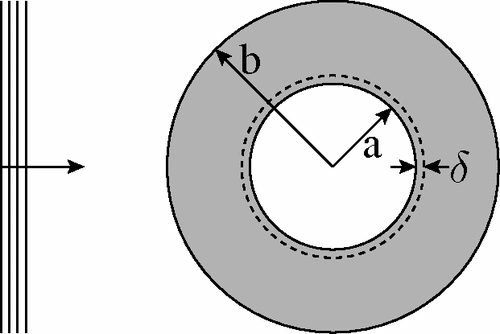
\includegraphics[height=0.15\paperheight]{1.png}
  \caption{Схема почти идеальной маскировочной оболочки: распределение параметров такое же, как идеальное, показанное в
  ур. \eqref{e2} и внешняя граница зафиксирована в $r=b$. Однако реальная внутренняя граница расположена в 
  $r=a +\delta$, где $\delta$ очень маленькое положительное число.}
  \label{fig:1}
\end{figure}

Отметим, что коэффициенты рассеяния не могут быть прямо получены для идеального плаща, так как $\varepsilon_\zeta \to 0,
\mu_r \to 0$ и $\mu_\theta \to \infty$, когда $r \to a$, и функции Бесселя второго рода в ур. \eqref{e7} имеют 
сингулярность при $r = a$. Чтобы обойти это мы вводим малое возмущение в идеальную оболочку, на такую оболочку будем
ссылаться как на почти идеальную, см. Рис.\ref{fig:1}.  Мы немного расширим внутреннюю границу так, что она будет
находится в $r = a + \delta$, где $\delta$ очень маленькое положительное число. Тем не менее, параметры все еще
вычисляются согласно формуле \eqref{e2}, как будто внутренняя граница не поменялась. Внешняя граница остается
зафиксированной $r = b$. Когда $\delta \to 0$ наша модель будет эквивалентна идеальной оболочке. Теперь электрическое
поле в каждой области задается соотношениями

\begin{equation*}
	(b<r)\mathbf{E}_\zeta = \sum\limits_l (\alpha_l^{in} \mathbf{J}_l(k_0 r)\exp(il\theta) +
								\alpha_l^{sc} \mathbf{H}_l(k_0 r)\exp(il\theta))
\end{equation*}
 
\begin{equation}\label{e10}
	(a+\delta<r<b)\mathbf{E}_\zeta = \sum\limits_l (\alpha_l^{1} \mathbf{J}_l(k_0 (r-a))\exp(il\theta) +
								\alpha_l^{2} \mathbf{H}_l(k_0 (r-a))\exp(il\theta))
\end{equation}

\begin{equation*}
	(r<a+\delta)\mathbf{E}_\zeta = \sum\limits_l \alpha_l^{3} \mathbf{J}_l(k_0 r)\exp(il\theta)
\end{equation*}
где $\alpha_l^i(i=1,2,3)$ коэффциенты разложения для результирующего поля внутри оболочки.

Касательные поля $\mathbf{E}_\zeta$ и $\mathbf{H}_\theta$(которое может быть получено из $\mathbf{E}_\zeta$)
должны быть непрерывны вдоль границы $r=a+\delta$ и $r=b$ и ортогональность $\exp(il\theta)$ позволяет волнам
в каждом порядке Бесселя разделяться. Таким образом, имеем следущие четыре уравнения:

\begin{align}
	& \alpha_l^{in} \mathbf{J}_l(k_0 b) + \alpha_l^{sc} \mathbf{H}_l(k_0 b) = 
	\alpha_l^1 \mathbf{J}_l(k_1(b-a)) + \alpha_l^2 \mathbf{H}_l(k_1(b-a)) \tag{\value{equation} a}\label{e11a}
\end{align}]

\begin{thebibliography}{99}
\bibitem{1}J. B. Pendry, D. Schurig, and D. R. Smith, Science 312, 1780 (2006).
\bibitem{2}U. Leonhardt, Science 312, 1777 (2006).
\bibitem{3}A. Alu and N. Engheta, Phys. Rev. E 72, 016623 (2005).
\bibitem{4}D. A. B. Miller, Opt. Express 14, 12457 (2006).
\bibitem{5}U. Leonhardt, New J. Phys. 8, 118 (2006).
\bibitem{6}S. A. Cummer, B. I. Popa, D. Schurig, D. R. Smith, and J. B. Pendry, Phys. Rev. E 74, 036621 (2006).
\bibitem{7}D. Schurig, J. J. Mock, B. J. Justice, S. A. Cummer, J. B. Pendry, A. F. Starr, and D. R. Smith, 
Science 314, 977 (2006).
\bibitem{8}G. W. Milton, M. Briane, and J. R. Willis, New J. Phys. 8, 248 (2006).
\bibitem{9}F. Zolla, S. Guenneau, A. Nicolet, and J. B. Pendry, Opt. Lett. 32, 1069 (2007).
\bibitem{10}W. Cai, U. K. Chettiar, A. V. Kildishev, and V. M. Shalaev, Nat. Photon. 1, 224 (2007).
\bibitem{11}H. Chen and C. T. Chan, Appl. Phys. Lett. 90, 241105 (2007).
\bibitem{12}H. C. van de Hulst, Light Scattering by Small Particles(Dover, New York, 1981).
\bibitem{13}D. Felbacq, G. Tayeb, and D. Maystre, J. Opt. Soc. Am. A 11, 2526 (1994).
\end{thebibliography}

\end{document}
